%%%%%%%%%%%%
%
% $Autor: Chantal Crety $
% $Datum: 11.07.2025 $
% $Pfad: DemonstratorSchrittmotor\DemontageAnleitung\Allgemein.tex
% $Beschreibung: Grundsätzliches für die DemontageAnleitung
%
%%%%%%%%%%%%

\chapter{Allgemeines}

Diese Demontageanleitung ist eng mit der Montageanleitung verknüpft, weshalb es zu inhaltlichen Überschneidungen kommen kann. Die Unterschiede liegen vor allem in der Reihenfolge der Arbeitsschritte.

\vspace{0.5em}
\textbf{Sicherheitshinweis:}\\
Stellen Sie bitte sicher, dass der Schrittmotor-Demonstrator stabil und standsicher steht und das Netzkabel gemäß den Angaben im Handbuch vollständig vom Stromnetz getrennt wurde, bevor Sie mit der Demontage beginnen.

\vspace{0.5em}
\textbf{Werkzeuge:}\\
Für die Demontage der elektrischen Komponenten empfehlen sich insbesondere folgende Werkzeuge: Ein Seitenschneider zum Durchtrennen von Kabelbindern, ein Cutter sowie ein Lötkolben zum Lösen von Lötverbindungen an den Schaltern.



\chapter{Demonstrator Bestandteile}

Um sich mit den verwendeten Bauteilen vertraut zu machen, werfen Sie bitte einen Blick auf die nachfolgende Übersicht der Gehäuseteile sowie die Materialliste.


\section{3D-Druckteile}
Die Konstruktion des Gehäuses besteht aus zwei Aufsteckplatten und zwei Gehäusehälften. Die Aufsteckplatten sind für den Bereich zwischen den Profilen vorgesehen und bilden zusammen mit der vorhandenen Steuerplatine samt Montageplatte eine Rückwand. Diese schützt die Elektronik vor Schmutz und bietet gleichzeitig eine Fläche zur Befestigung elektronischer Komponenten.
Die Gehäusehälften bieten Platz für die Kabelführung, schützen das Innenleben und halten alle wichtigen Elemente sicher in Position.

\begin{minipage}{0.48\textwidth}
	\begin{figure}[H]
		\centering
		\begin{tikzpicture}[scale=1.4]
			\tikzstyle{every node}=[font=\LARGE]
			\draw [line width=1pt, short] (5.25,10.5) -- (5.5,10.5);
			\draw [line width=1pt, short] (5.5,7.5) -- (5.75,7.5);
			\draw [line width=1pt, short] (5.5,10.5) -- (5.75,7.5);
			\draw [line width=1pt, short] (5.25,10) -- (5,10);
			\draw [line width=1pt, short] (5.25,10.5) -- (5,10.5);
			\draw [line width=1pt, short] (5,10) -- (5,10.5);
			\draw [line width=1pt, short] (5,10.5) -- (5.5,10.75);
			\draw [line width=1pt, short] (5.5,10.75) -- (5.75,10.75);
			\draw [line width=1pt, short] (7.25,11.75) -- (7.75,12);
			\draw [line width=1pt, short] (5.25,7.5) -- (5.5,7.5);
			\draw [line width=1pt, short] (5.25,7.75) -- (5.25,7.5);
			\draw [line width=1pt, short] (5.25,7.75) -- (5.5,7.75);
			\draw [line width=1pt, short] (5.25,7.75) -- (5.5,8);
			\draw [line width=1pt, short] (5.5,7.75) -- (5.25,10);
			\draw [line width=1pt, short] (5.75,7.5) -- (8.5,9.25);
			\draw [line width=1pt, short] (8.5,9.25) -- (8.25,12);
			\draw [line width=1pt, short] (5.5,10.5) -- (8.25,12);
			\draw [line width=1pt, short] (7.75,12) -- (8.25,12);
			\draw [line width=1pt, short] (5.75,10.75) -- (7.5,11.75);
			\draw [line width=1pt, short] (7.25,11.75) -- (7.5,11.75);
		\end{tikzpicture}
		\caption{Platte groß}
		\label{fig:platte_gross}
	\end{figure}
\end{minipage}
\hfill
\begin{minipage}{0.48\textwidth}
	\begin{figure}[H]
		\centering
		\begin{tikzpicture}[scale=0.6]
			\tikzstyle{every node}=[font=\LARGE]
			\draw [line width=1pt, short] (10,5.25) -- (10.25,-2);
			\draw [line width=1pt, short] (10,5.25) -- (15,7.75);
			\draw [line width=1pt, short] (10.25,-2) -- (15.25,1);
			\draw [line width=1pt, short] (15.25,1) -- (15,7.75);
			\draw [line width=1pt, short] (10,5.25) -- (9.25,5.5);
			\draw [line width=1pt, short] (15,7.75) -- (14.25,8);
			\draw [line width=1pt, short] (10.25,-2) -- (9.5,-1.5);
			\draw [line width=1pt, short] (9.5,-0.75) -- (9.5,-1.5);
			\draw [line width=1pt, short] (9.5,-0.75) -- (9.75,-1);
			\draw [line width=1pt, short] (9.5,4.75) -- (9.75,-1);
			\draw [line width=1pt, short] (9.25,5.5) -- (9.25,4.5);
			\draw [line width=1pt, short] (9.25,4.5) -- (9.5,4.75);
			\draw [line width=1pt, short] (9.25,5.5) -- (10.25,6);
			\draw [line width=1pt, short] (14.25,8) -- (13.25,7.5);
			\draw [line width=1pt, short] (13.25,7.5) -- (13.5,7.5);
			\draw [line width=1pt, short] (13.5,7.5) -- (10.5,6);
			\draw [line width=1pt, short] (10.25,6) -- (10.5,6);
			\draw [line width=1pt, short] (9.5,-0.75) -- (9.75,-0.5);
			\draw [line width=1pt] (12.25,3.75) ellipse (0.25cm and 0.25cm);
			\node [font=\LARGE] at (12.75,3.75) {};
			\draw [line width=1pt] (12.25,2) ellipse (0.25cm and 0.25cm);
			\draw [line width=1pt, short] (12.25,4) .. controls (12.5,3.75) and (12.25,3.75) .. (12.25,3.5);
			\draw [line width=1pt, short] (12.25,2.25) .. controls (12.5,2) and (12.25,2) .. (12.25,1.75);
		\end{tikzpicture}
		\caption{Platte klein}
		\label{fig:platte_klein}
	\end{figure}
\end{minipage}

\vspace{0.5cm}

\begin{figure}[H]
	\centering
	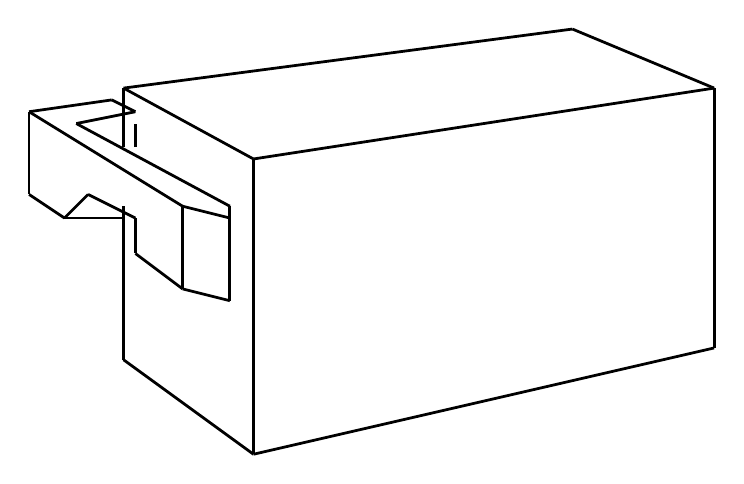
\begin{tikzpicture}[scale=0.6]
		\tikzstyle{every node}=[font=\LARGE]
		\draw [line width=1pt] (10.5,2.75) -- (20.25,5);
		\draw [line width=1pt] (5.75,10) -- (7.5,10.25);
		\draw [line width=1pt] (5.75,10) -- (9,8);
		\draw [line width=1pt] (9,8) -- (9,6.25);
		\draw [line width=1pt] (5.75,10) -- (5.75,8.25);
		\draw [line width=1pt] (10,8) -- (6.75,9.75);
		\draw [line width=1pt] (6.75,9.75) -- (8,10);
		\draw [line width=1pt] (7.5,10.25) -- (8,10);
		\draw [line width=1pt] (7.75,4.75) -- (7.75,7);
		\draw [line width=1pt] (8,9.25) -- (8,9.75);
		\draw [line width=1pt] (7.75,4.75) -- (10.5,2.75);
		\draw [line width=1pt] (10.5,2.75) -- (10.5,9);
		\draw [line width=1pt] (10.5,9) -- (20.25,10.5);
		\draw [line width=1pt] (20.25,5) -- (20.25,10.5);
		\draw [line width=1pt] (7.75,10.5) -- (7.75,9.25);
		\draw [line width=1pt] (6.5,7.75) -- (7,8.25);
		\draw [line width=1pt] (7,8.25) -- (8,7.75);
		\draw [line width=1pt] (8,7.75) -- (8,7);
		\draw [line width=1pt] (6.5,7.75) -- (5.75,8.25);
		\draw [line width=1pt] (8,7) -- (9,6.25);
		\draw [line width=1pt] (6.5,7.75) -- (7.75,7.75);
		\draw [line width=1pt] (7.75,8) -- (7.75,7);
		\draw [line width=1pt] (10.5,9) -- (7.75,10.5);
		\draw [line width=1pt] (7.75,10.5) -- (17.25,11.75);
		\draw [line width=1pt] (20.25,10.5) -- (17.25,11.75);
		\draw [line width=1pt] (9,6.25) -- (10,6);
		\draw [line width=1pt] (9,8) -- (10,7.75);
		\draw [line width=1pt] (10,7.75) -- (10,6);
		\draw [line width=1pt] (10,8) -- (10,7.75);
	\end{tikzpicture}
	
	\caption{Körper links}
	\label{tikz:Kl}
\end{figure}

\begin{figure}[H]
	\vspace{0.5cm}
	\centering
	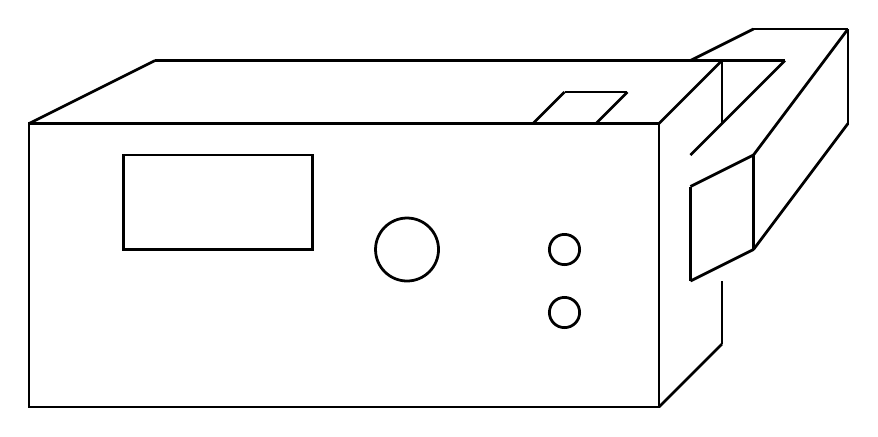
\begin{tikzpicture}[scale=1.6]
		\tikzstyle{every node}=[font=\LARGE]
		\draw[line width=1pt] (5,11) rectangle (10,8.75);
		\draw [line width=1pt] (10,11) -- (10.5,11.5);
		\draw [line width=1pt] (10,8.75) -- (10.5,9.25);
		\draw [line width=1pt] (10.25,10.75) -- (11,11.5);
		\draw [line width=1pt] (11,11.5) -- (10.5,11.5);
		\draw [line width=1pt] (10.25,11.5) -- (10.75,11.75);
		\draw [line width=1pt] (10.75,11.75) -- (11.5,11.75);
		\draw [line width=1pt] (11.5,11.75) -- (10.75,10.75);
		\draw [line width=1pt] (10.75,10.75) -- (10.25,10.5);
		\draw [line width=1pt] (10.25,10.5) -- (10.25,9.75);
		\draw [line width=1pt] (10.25,9.75) -- (10.75,10);
		\draw [line width=1pt] (10.75,10.75) -- (10.75,10);
		\draw [line width=1pt] (10.75,10) -- (11.5,11);
		\draw [line width=1pt] (11.5,11.75) -- (11.5,11);
		\draw [line width=1pt] (10.5,11.5) -- (10.5,11);
		\draw [line width=1pt] (5,11) -- (6,11.5);
		\draw [line width=1pt] (10.5,11.5) -- (6,11.5);
		\draw [line width=1pt] (10.5,9.75) -- (10.5,9.25);
		\draw [line width=1pt] (9,11) -- (9.25,11.25);
		\draw [line width=1pt] (9.25,11.25) -- (9.75,11.25);
		\draw [line width=1pt] (9.25,11.25) -- (9.5,11.25);
		\draw [line width=1pt] (9.75,11.25) -- (9.5,11);
		\draw [line width=1pt] (9.25,11.25) -- (9.75,11.25);
		\draw[line width=1pt] (8,10) circle (0.25cm);
		\draw[line width=1pt] (9.25,10) circle (0.12cm);
		\draw[line width=1pt] (9.25,9.5) circle (0.12cm);
		\draw[line width=1pt] (5.75,10.75) rectangle (7.25,10);
		\draw [line width=1pt] (9.25,11.25) -- (9.5,11.25);
		\draw [line width=1pt] (9.5,11.25) -- (9.75,11.25);
		\draw [line width=1pt] (9.25,11) -- (9.5,11);
		\draw [line width=1pt] (9.25,11) -- (9.5,11);
	\end{tikzpicture}
	\caption{Körper rechts}
	\label{tikz:KR}
\end{figure}


\section{Materialliste}

\begin{center}
	\scriptsize
	\begin{longtable}{|c|c|p{2.5cm}|p{2cm}|p{0.8cm}|c|p{2cm}|}
		
		\hline
		\textbf{Pos.} & \textbf{Stk.} & \textbf{Bezeichnung} & \textbf{Artikel-Nr.} & \textbf{Preis [€]} & \textbf{Abbildung} & \textbf{Bestelladresse} \\
		\hline
		1 & 1 & Genmitsu 3018 Pro CNC Fräsemachine & 101-60-280PRO & 219,00  & 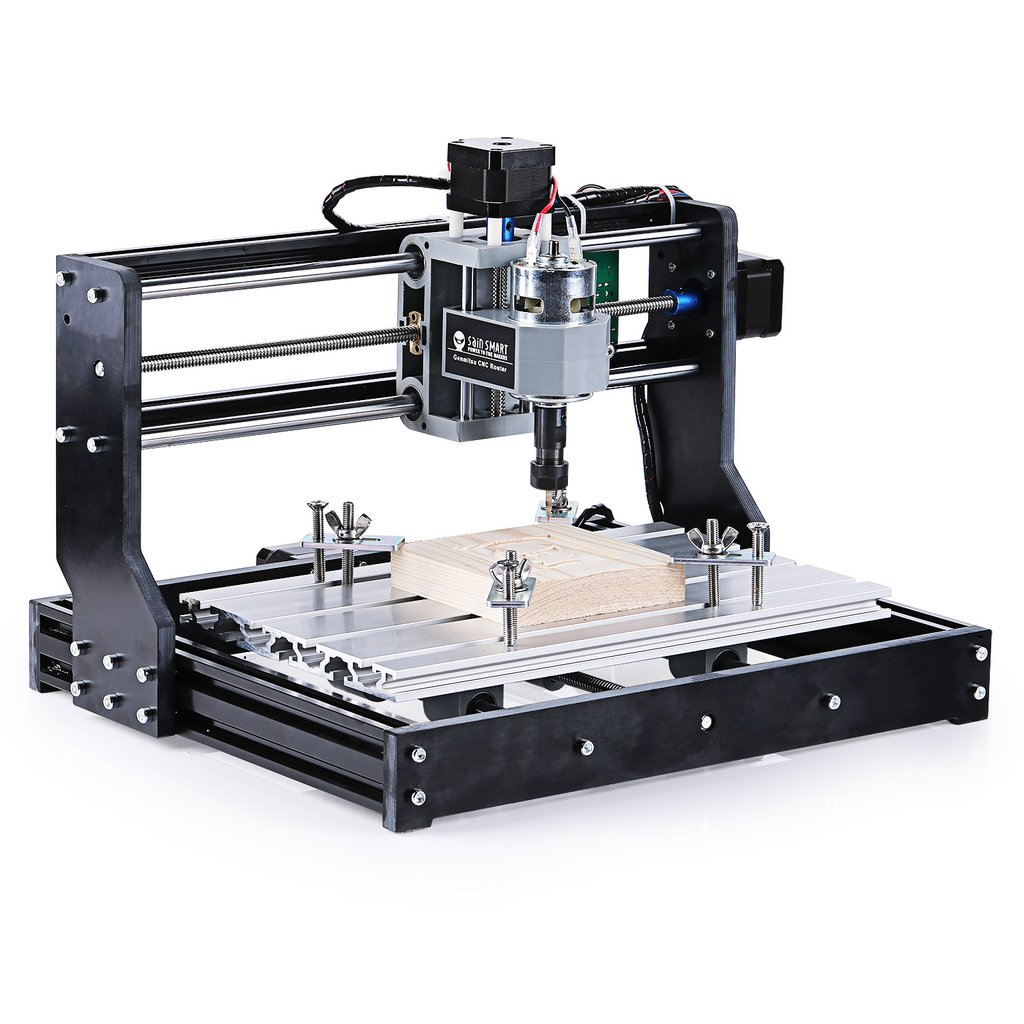
\includegraphics[width=1.5cm]{Images/fraesmaschine.jpg}
		& \url{www.amazon.de} \\
		\hline
		2 & 1 & Arduino Nano 33 BLE Sense Rev.2\newline nRF52840, mit Header& ARD NANO 33BSH2 & 47,70 & 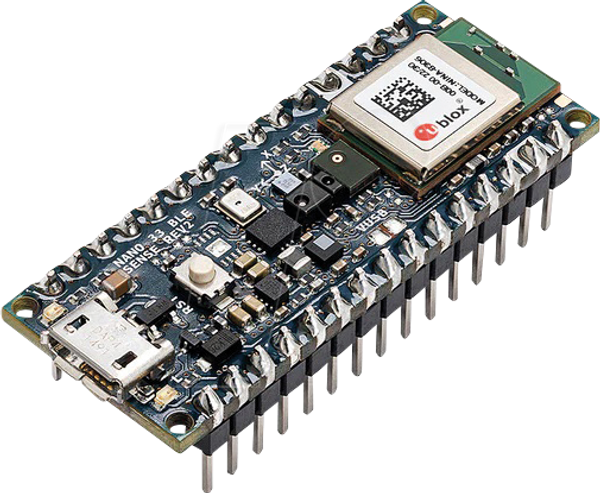
\includegraphics[width=1.5cm]{Images/arduino.png} & \url{www.reichelt.de} \\
		\hline
		5 & 1 & 65 Jumper Wire Kabel im Set & RBS10022 & 1,55 & 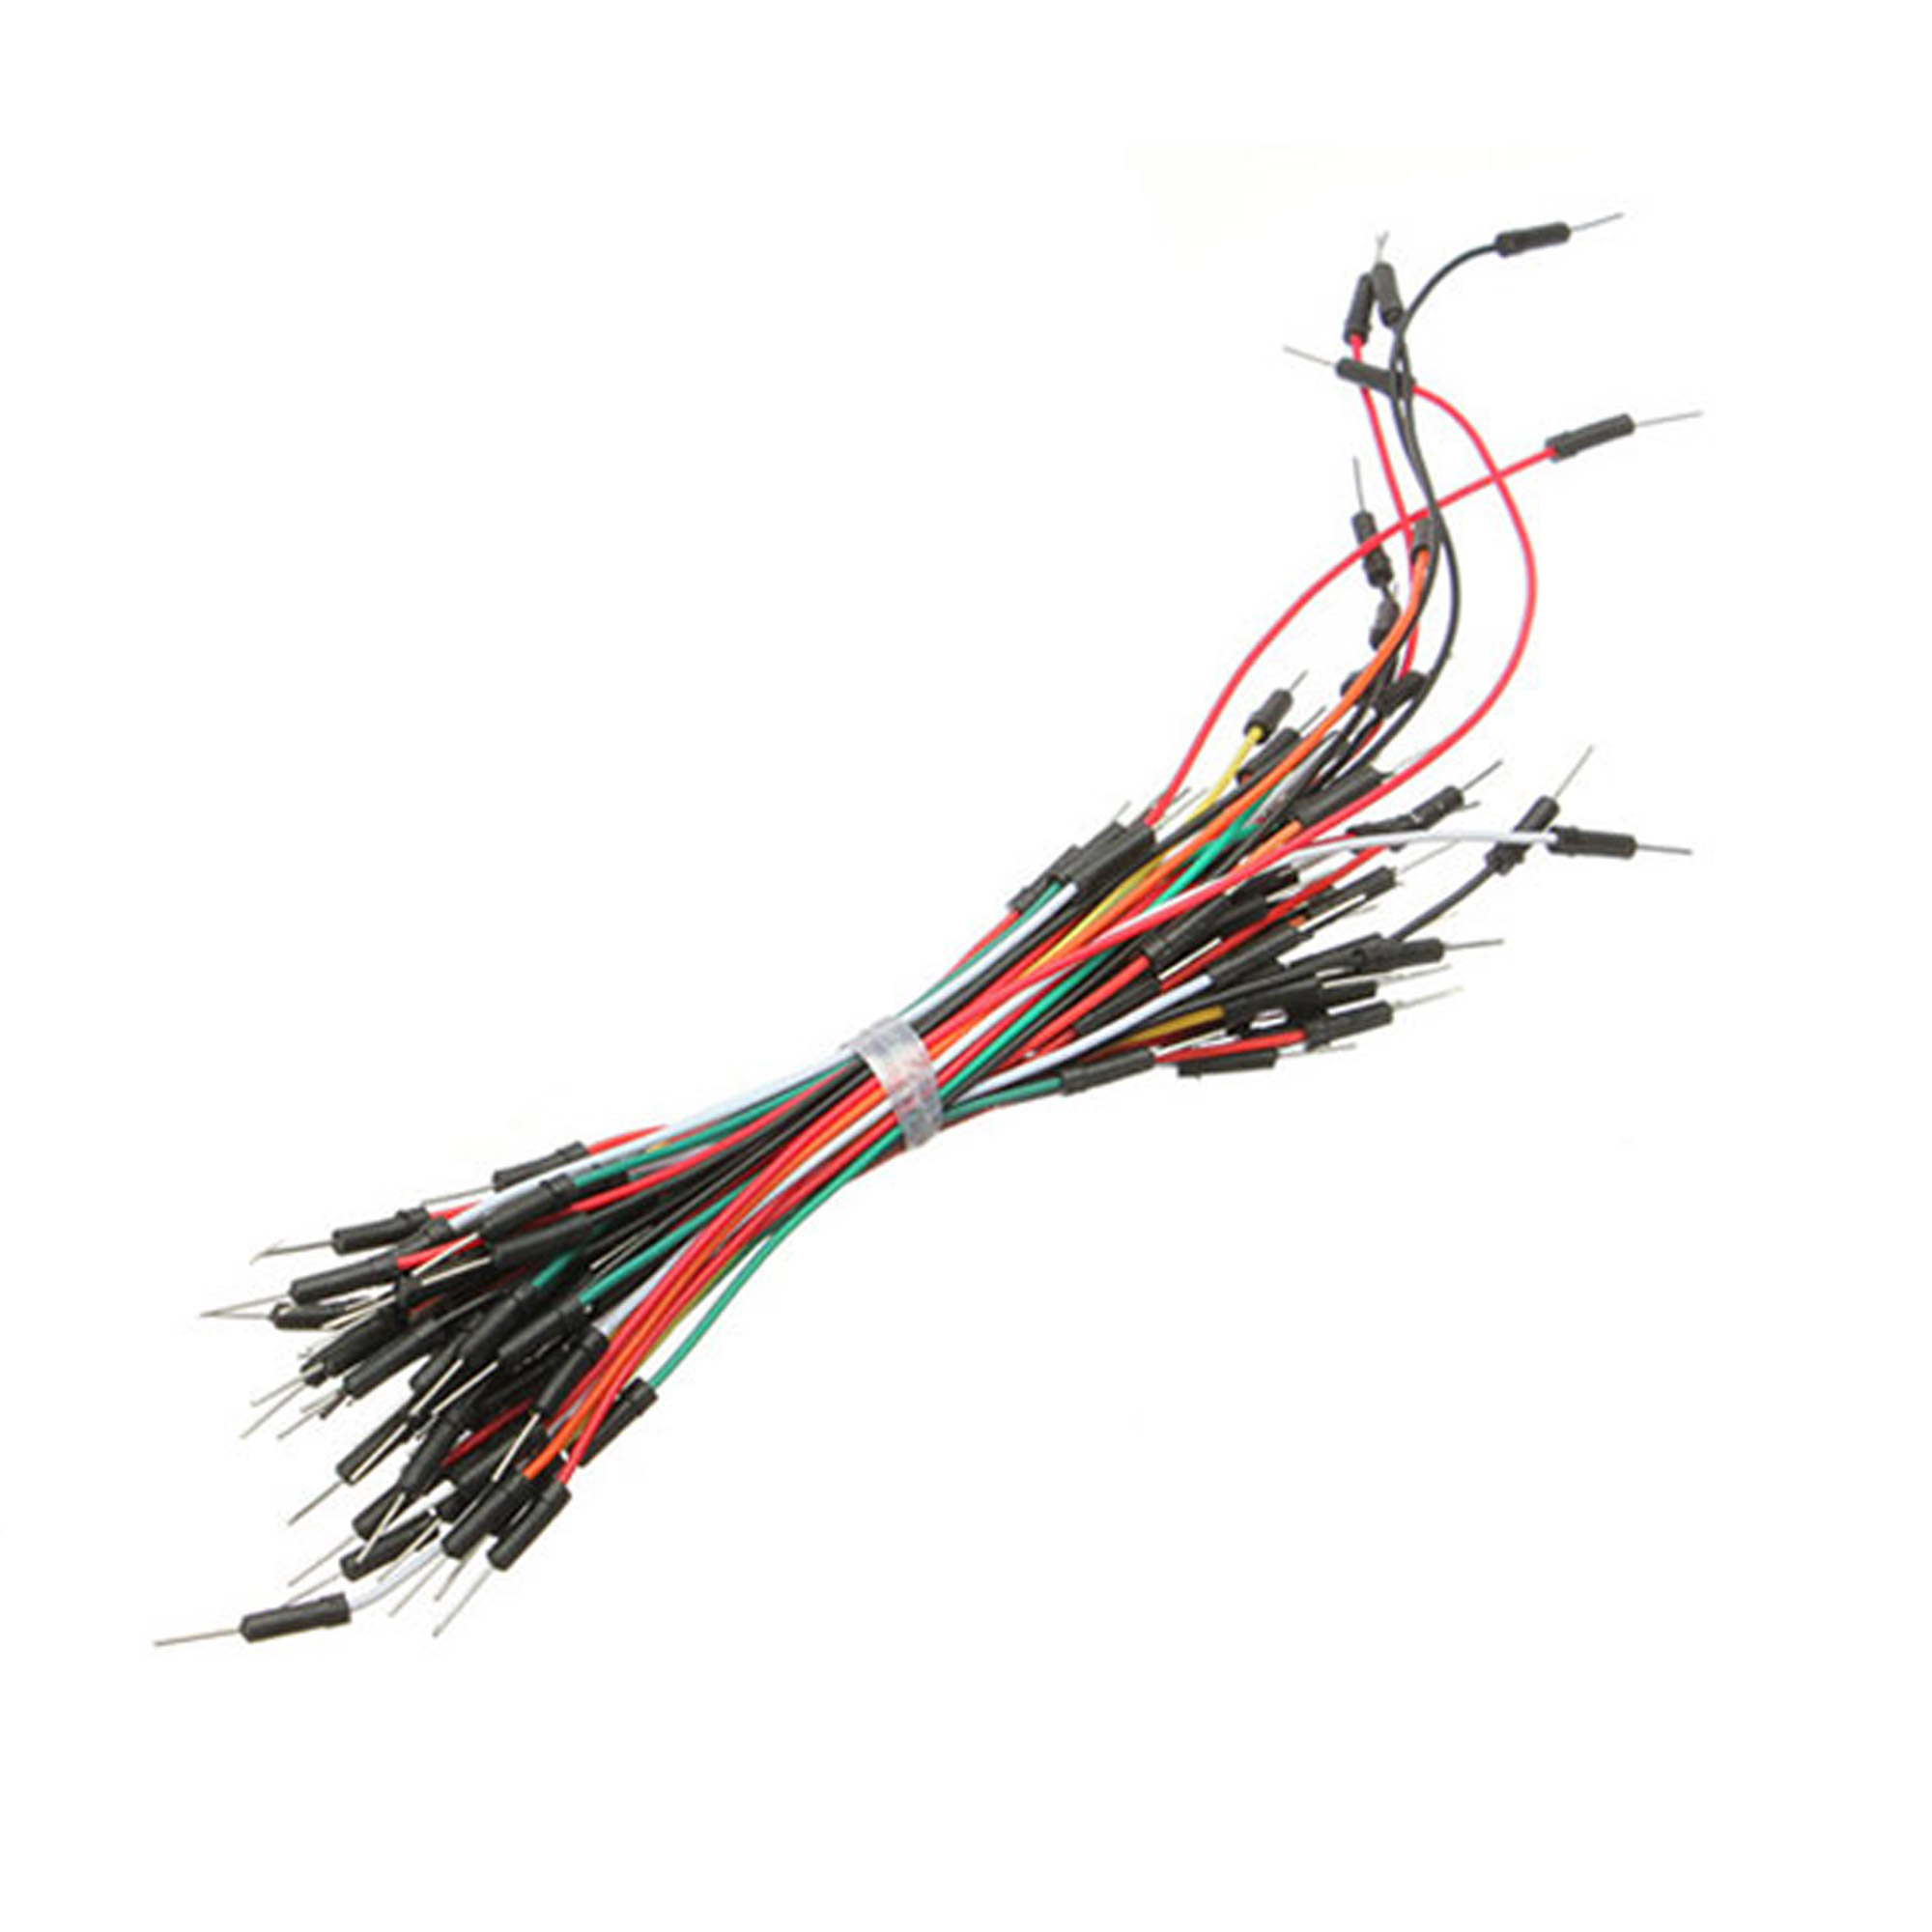
\includegraphics[width=1.5cm]{Images/jumpercablemm.jpg} & \url{www.roboter-bausatz.de} \\
		\hline
		4 & 1 & 40 Pin Dupont / Jumper Kabel Buchse-Buchse 20 cm & RBS101126 & 0,98 & 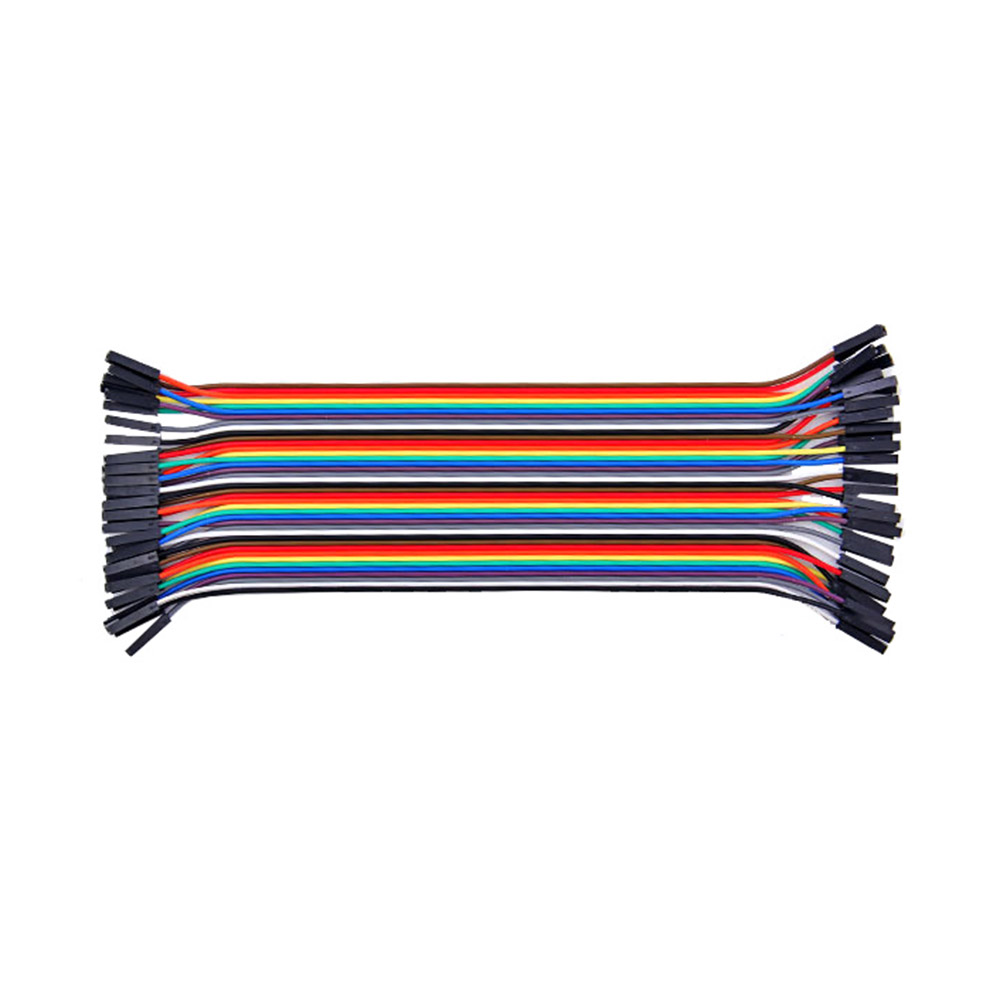
\includegraphics[width=1.5cm]{Images/jumpercableff.jpg} & \url{www.roboter-bausatz.de} \\
		\hline
		5 & 1 & 40 Pin Jumper Kabel Buchse-Stecker 20 cm & RBS10028 & 1,15 & 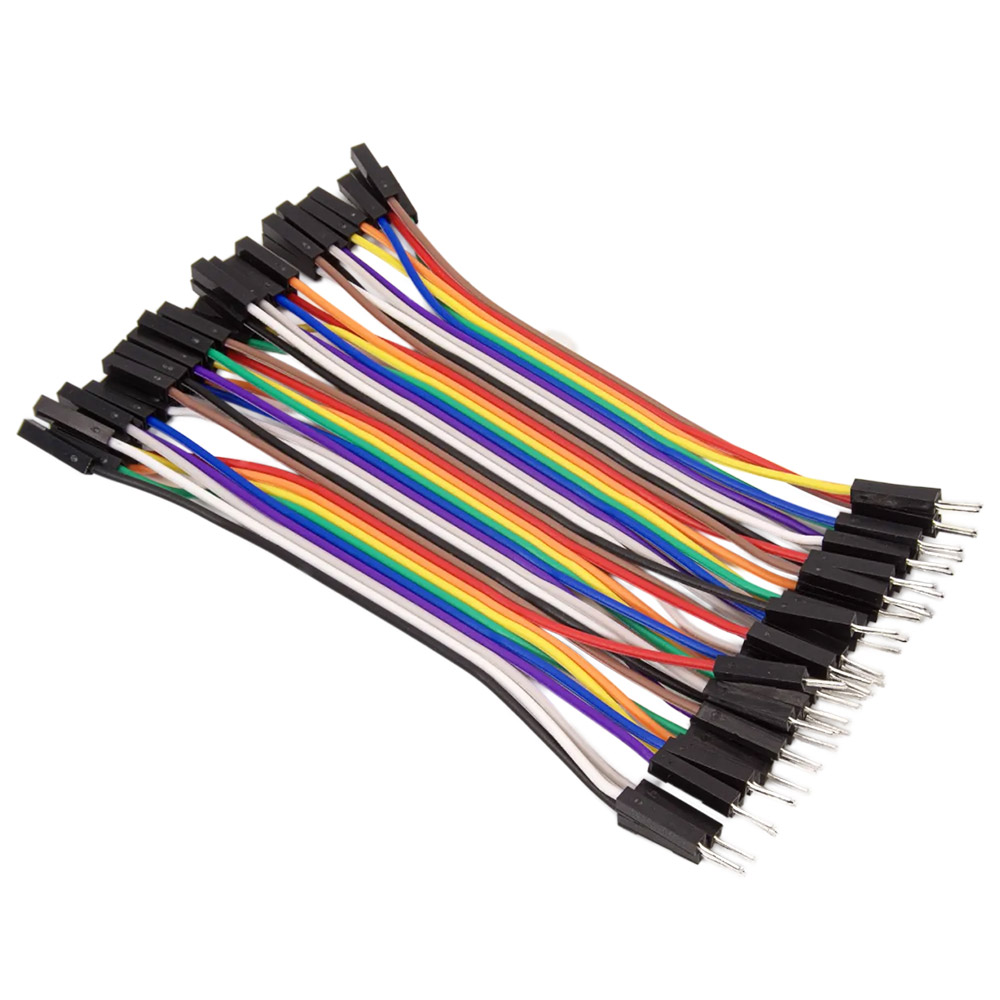
\includegraphics[width=1.5cm]{Images/jumpercablemf.jpg} & \url{www.roboter-bausatz.de} \\
		\hline
		6 & 1 & Arduino - Grove Universal-Kabel, 4-Pin, 20 cm & GRV CA-BLE4PIN20 & 2,50 & 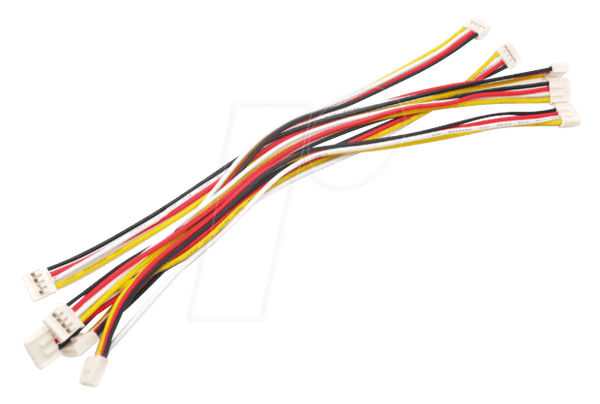
\includegraphics[width=1.5cm]{Images/grove2.png} & \url{www.reichelt.de} \\
		\hline
		7 & 1 & TRU COMPONENTS DC-13M Niedervolt-Steckverbinder Stecker, gerade 5.5 mm 2.5 mm 1 St. & 1572162 - VQ & 3,79 & 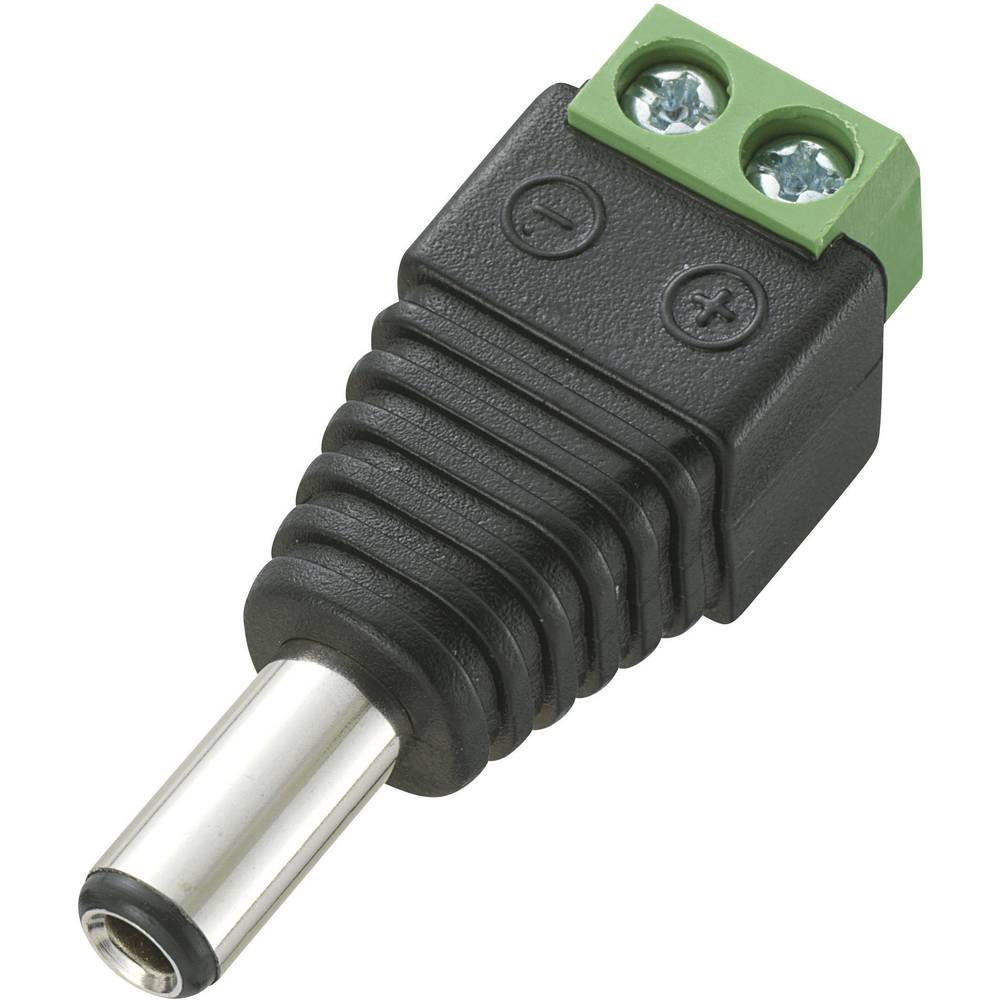
\includegraphics[width=1.5cm]{Images/schutzstecker.jpg} & \url{www.conrad.de} \\
		\hline
		8 & 1 & Steckernetzteil, 12 W, 12 V, 1 A & NKSK 200 SW GEW & 3,10 & 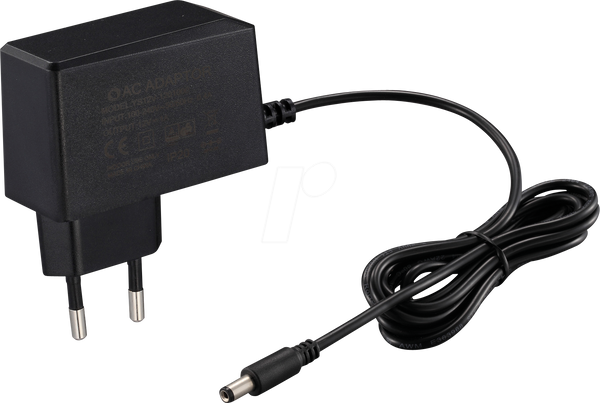
\includegraphics[width=1.5cm]{Images/netzteil.png} & \url{www.reichelt.de} \\
		\hline
		9 & 1 & Drucktaster 0,1A-24VAC 1x (Ein) Ø11/9,1mm rt & RAFI 107.301 & 2,99 & 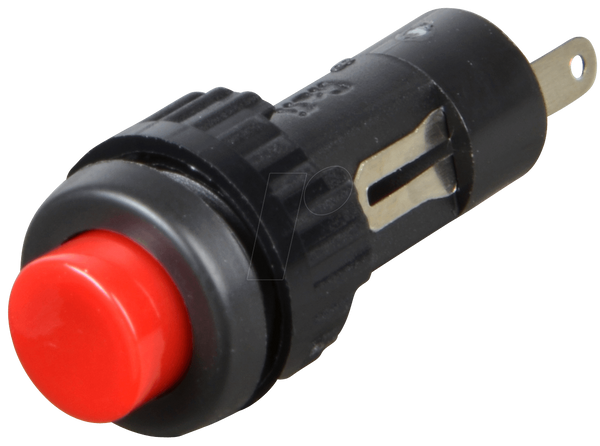
\includegraphics[width=1.5cm]{Images/tasterr.png} & \url{www.reichelt.de} \\
		\hline
		10 & 1 & Drucktaster 0,1A-24VAC 1x (Ein) Ø11/9,1mm gn & RAFI 107.507
		& 2,90 & 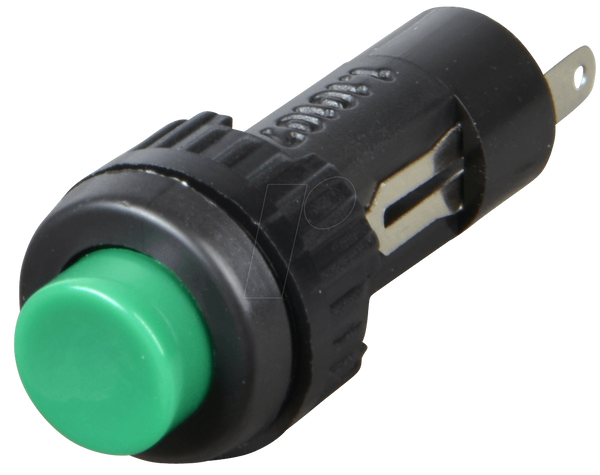
\includegraphics[width=1.5cm]{Images/tasterg.png} & \url{www.reichelt.de} \\
		\hline
		11 & 2 & Snap-Action-Mikroschalter, 1x UM, Rollenhebel & AV 32543 AT & 1,80 & 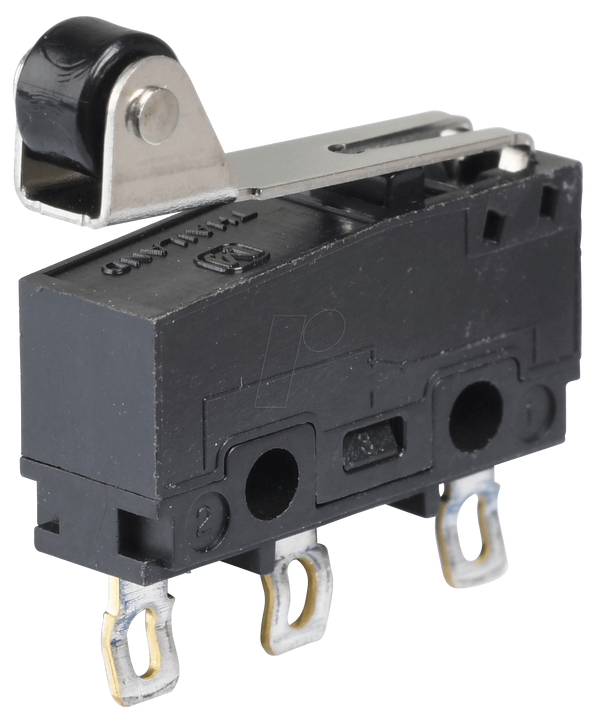
\includegraphics[width=1.5cm]{Images/microschalter.png} & \url{www.reichelt.de} \\
		\hline
		12 & 1 & Entwicklungsboard mit DRV8825 Motortreiber & DEBO DRV A4988 & 5,80 & 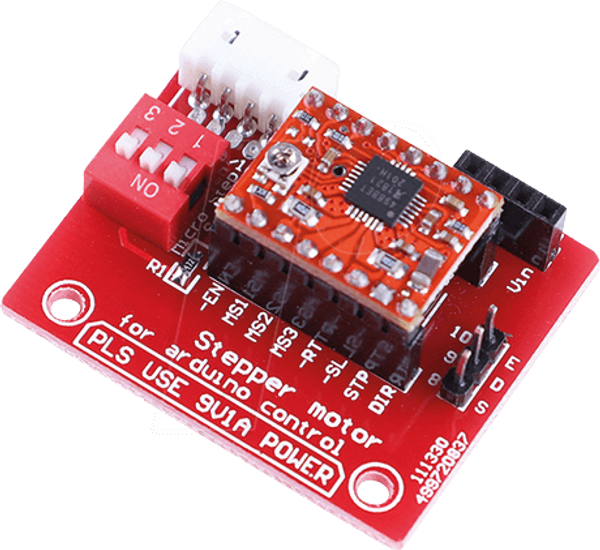
\includegraphics[width=1.5cm]{Images/treiber.png} & \url{www.reichelt.de} \\
		\hline
		13 & 1 & Entwicklerboards - Display OLED, 2,42", 128x64 Pixel & DEBO OLED 2.42 & 18,90 & 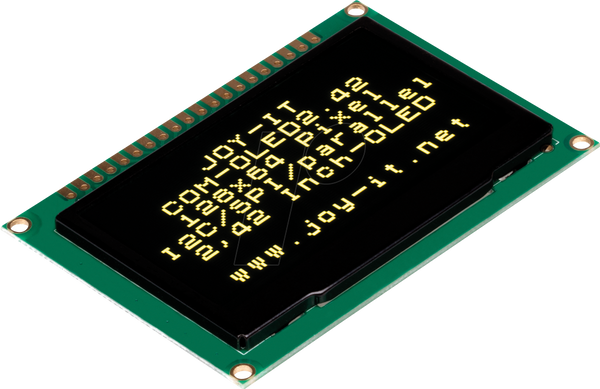
\includegraphics[width=1.5cm]{Images/display.png} & \url{www.reichelt.de} \\
		\hline
		14 & 1 & Sunlu PLA Filament 0.75mm 1kg & RBS16624 & 17,95 & 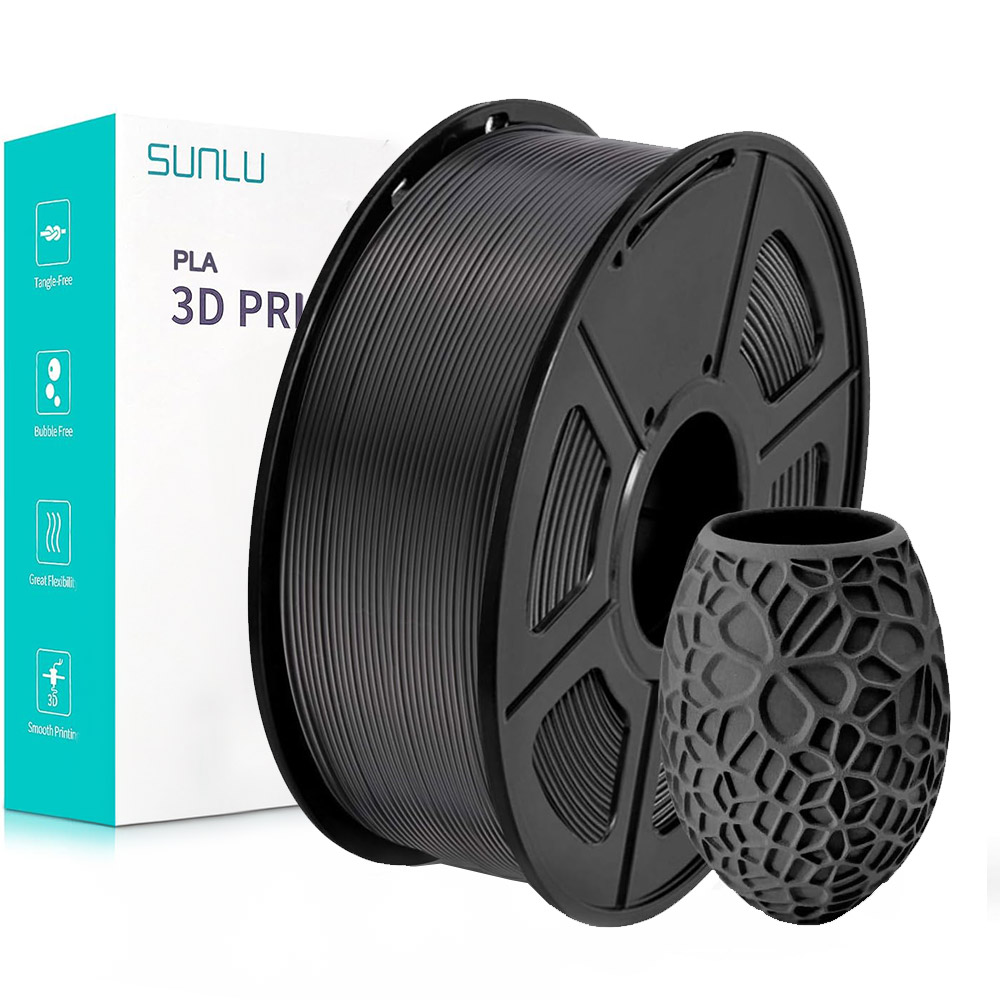
\includegraphics[width=1.5cm]{Images/filament.jpg} & \url{www.roboter-bausatz.de} \\
		\hline
		15 & 1 & Experimentier-Slide-Steckboard, 300/100 Kontakte & STECKBOARD S4 & 4,20 & 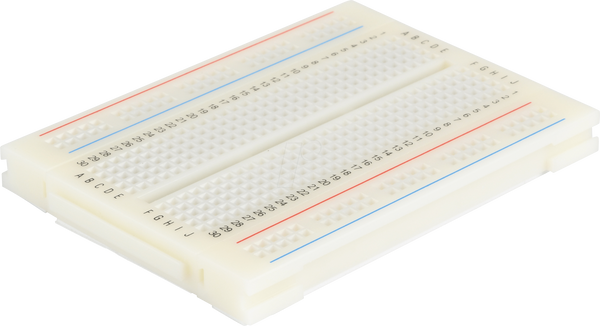
\includegraphics[width=1.5cm]{Images/breadboard.png} & \url{www.reichelt.de} \\
		\hline
		16 & 1 & Kabelbinder-Set, verschiedene Größen, mehrfarbig, 200er-Pack & DELOCK 18628 & 3,85 & 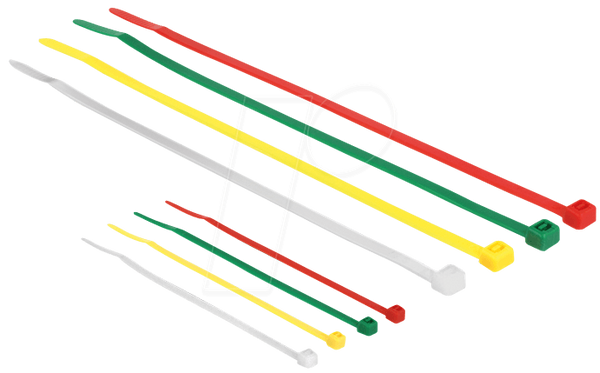
\includegraphics[width=1.5cm]{Images/kabelbinder.png} & \url{www.reichelt.de} \\
		\hline
		17 & 1 & Drehwinkel-Encoder, KY-040 & DEBO ENCODER & 2,20 & 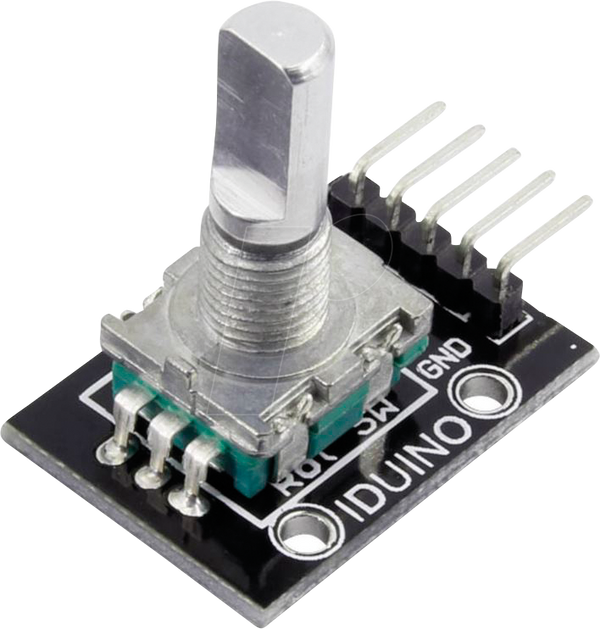
\includegraphics[width=1.5cm]{Images/drehknopf.png} & \url{www.reichelt.de} \\
		\hline
		18 & 1 & Wippschalter, 2x Aus, schwarz, I-O & WIPPE 1858.1103 & 2,60 & 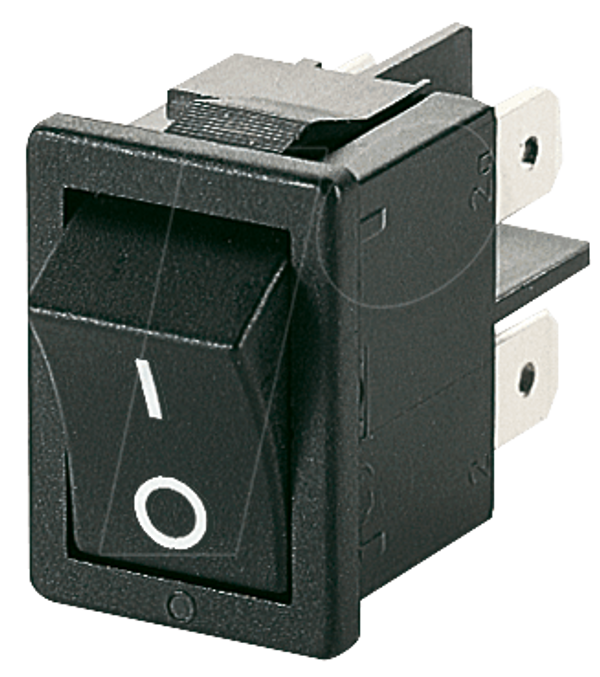
\includegraphics[width=1.5cm]{Images/wippschalter.png} & \url{www.reichelt.de} \\
		\hline
		19 & 1 & Zylinderkopfschraube, Sechskantschraube, M5, 10 mm & ZS M5X10 & 0,30 & 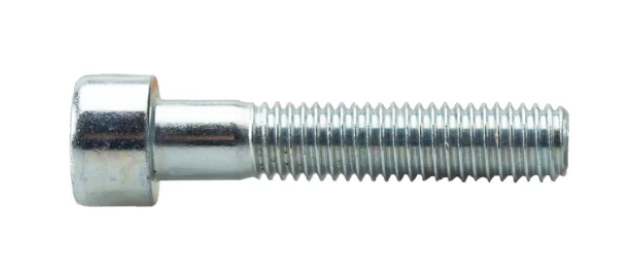
\includegraphics[width=1.5cm]{Images/zylinderkopfschraube.png} & \url{www.reichelt.de} \\
		\hline
		20 & 3 & Flach-Senkkopfschrauben, Kreuzschlitz, M3, 10 mm & SKS M3X10-50 & 1,75 & 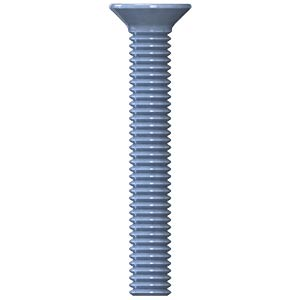
\includegraphics[width=1.5cm]{Images/senkkopfschraube.jpg} & \url{www.reichelt.de} \\
		\hline
		21 & 3 & Sechskantmuttern, Edelstahl A2, M3 & SK-E M3-100 & 4,55 & 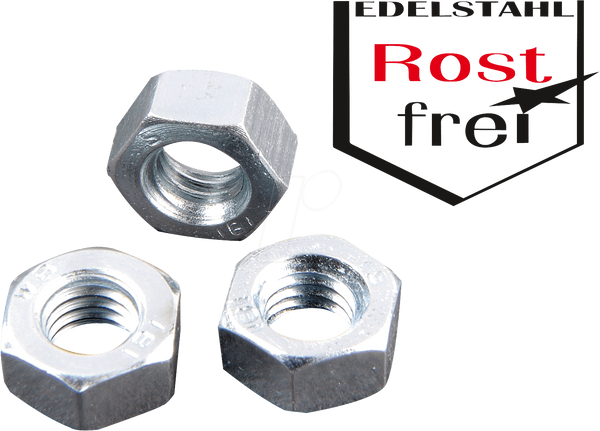
\includegraphics[width=1.5cm]{Images/muttern.png} & \url{www.reichelt.de} \\
		\hline	
		22 & 1& Unterlegscheiben, 10,5 mm & SKU 10,5-100 & 5,35 & 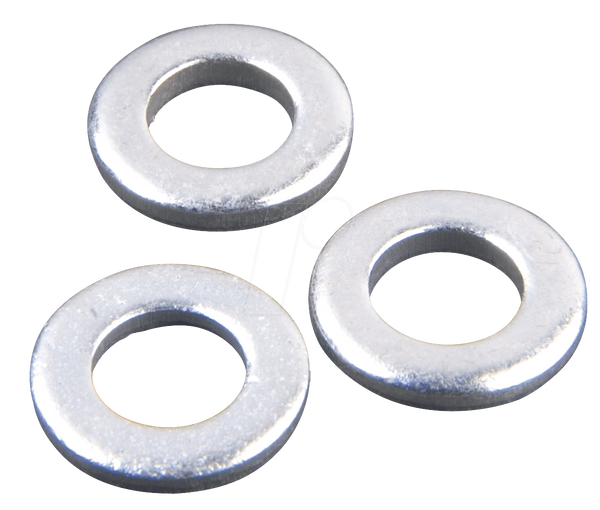
\includegraphics[width=1.5cm]{Images/unterlegscheibe.png} & \url{www.reichelt.de} \\
		\hline
		23 & 1& Elektroniklot EL 324 bleifrei 70 g & CFH 52324 & 10,99 & 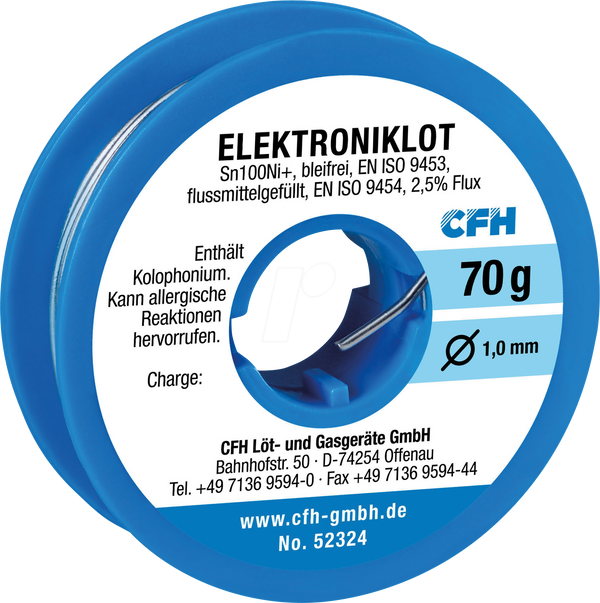
\includegraphics[width=1.5cm]{Images/loetzinn.png} & \url{www.reichelt.de} \\
		\hline	
		
		\caption{Gesamtliste}
		\label{tab:Gesamtliste}
		
	\end{longtable}
\end{center}
